%\section{Introduction}
%\label{sec:intro}

%\section{Basics}
%\labe{sec:basics}

%\section{Related Work}
%\label{sec:related_work}
\section{Introduction}
\label{Introduction}

One of the central objectives in the area of artificial intelligence (AI) is to create fully autonomous agents. These systems should improve over time through trial and error, so the trained agents will eventually know the optimal behaviour when interacting with their environment \cite{brundage17}. Reinforcement learning (RL) is a principled mathematical framework to achieve experience-based autonomous learning \cite{strehl09}.\\
In recent years, RL methods have driven impressive advances in AI, achieving superhuman performance in numerous domains \cite{chessSilver2017mastering, GoalphaGosilver2017mastering}. Several of these advances have been achieved by combining RL with deep learning techniques. Especially for problems with high dimensional state-space, this combination has proven to be powerful \cite{lavet18}.
Despite revolutionary progress, limitations still exists due to memory complexity, computational complexity and sample complexity \cite{strehl09}. Therefore, some applications require a level of knowledge that surpasses the capabilities achieved by AI.\\
Autonomous driving is one example \cite{sallab17}. The car has to interact strongly with its complex environment (e.g. other vehicles, pedestrians, roadworks) and will only be brought on the market if it is near to risk free. The straight-forward idea of solving these problems would be end-to-end supervised learning. This approach usually demands massive amount of labelled data and consequently requires significant (time consuming) human involvement. By contrast, RL typically learns by trial-and-error and does not need explicit human supervision \cite{you17}. Still, due to the high complexity and safety issues of autonomous driving, training and testing with standard RL trial-and-error methods may be prohibitively expensive and time consuming \cite{uesato18}.\\
To enhance RL algorithms, biologically influenced extensions of the basic concept have emerged from recent studies \cite{environmentBansal2017Oct, gabor19, robustPinto2017Mar, uesato18}. Some inspiration derived from predator-prey relationships, which are often observed in biology. Both evolutionary processes try to influence each others fitness (co-evolution). The predator tries to maximize its reward by eating the prey, while the prey wants to achieve the exact opposite. Theoretically, when antagonistic populations are trying to outperform each other, it may result in fast improvements and increased genetic robustness \cite{berenos10}. This natural phenomenon is called competitive co-evolution and can be transferred to evolutionary algorithms \cite{gabor19}.\\
In this paper, we exclusively focus on concepts of competitive co-evolutionary and adversarial learning. First, we introduce the basic concepts (chapter \ref{Basics}) needed to understand said concepts. Then, we present and compare different state of the art adversarial and co-evolutionary algorithms for training (chapter \ref{adv_training}) and testing (chapter \ref{testing}) reinforcement learning agents.
\begin{comment}
THOMY:

- Basics?
was rein?
	- reinforcement learning? - auf jeden fall
    - deep neural networks? - deep reinforcement learning (reinforcement mit neuronalen netzen) (q-learning)
    - value network vs policy network - nein
    - monte-carlo-search-trees - nein 
    - PPO (proximal policy optimization) - nein
    - zero sum games (!) - definition - konsistente notation 
    
    - Formeln (markov decision processes)

\end{comment}

\section{Basics}
\label{Basics}

\subsection{Markov Decision Processes}
\label{mdp}

Markov Decision Processes (MDP) \cite{gabor19, puterman94} are a class of sequential decision processes and described via the tuple $M = \langle S, A, P, R \rangle$, where
\begin{description}
   \begin{itemize}
        \item $S$ is a finite set of states and $s_t \in S$ the state of the MDP at time step $t$. 
        \item $A$ is the set of actions and $a_t \in A$ the action the MDP takes at time step $t$.
        \item $P(s_{t+1}|s_t,a_t)$ is the probability transition function. It describes the transition that occurs when action $a_t$ is executed in state $s_t$. The resulting state $s_{t+1}$ is chosen according to $P$.
        \item $R(s_t,a_t)$ is the reward, when the MDP takes action $a_t$ in state $s_t$. We assume $R(s_t,a_t) \in \mathbb{R}$
   \end{itemize}
\end{description}
Consequently, the cost and transition functions only depend on the current state and action of the system. Eventually, the MDP should find a policy $\pi : S \rightarrow A$ which maximizes the return $G_t$ at state $s_t$ over an infinite horizon via:
\begin{equation}
    G_t = \sum_{k=0}^\infty \gamma^k \cdot R(s_{t+k}, a_{t+k})
\end{equation}
, with $\gamma \in [0,1]$ as the discount factor. The optimal policy is a policy that returns a higher $G_t$ than all other policies.

\subsection{Reinforcement Learning}
\label{reinforcement}
The goal is to search the policy space $\Pi$ with model-free reinforcement learning \cite{strehl09} to find the optimal policy $\pi^*$. We model the Reinforcement Learning problem as a MDP environment with a finite state and action space. The reinforcement learning agent executes an action $a_t$ for every timestep $t \in [1,..]$ in the MDP environment. In model-free algorithms, the agent acts without any knowledge of the environment and the algorithm only keeps value-function information. Therefore, the agents knows its current state $s_t$ and the action space $A$, but neither the reward nor the next state $s_{t+1}$ of any action $a_t$ in any space $s_t$.\\
Consequently, the agent needs to learn from delayed rewards without having a model of the environment. A popular value-based approach to solve this problem is Q-learning \cite{peng04}. Policies $\pi$ and the action-value function $Q^{\pi} : S \times A \rightarrow \mathbb{R},\pi \in \Pi$ are represented by a two-dimensional lookup table indexed by state-action pairs. The action-value function describes the expected total discounted return $Q^{\pi}(s_t,a_t)$ when taking action $a_t$ in state $s_t$ and following policy $\pi$ for all later states $s_t, s_{t+1},..$ afterwards.\\
We start with an initial guess of $Q$, which will be continually updated to get the optimal state-value function $Q^*$ after time.

%\begin{comment}

\begin{comment}

\subsection{Q-Learning in Deep neural networks}
\label{qlearn}
Reinforcement learning (\ref{reinforcement}) can be done using neural networks. in this section we first introduce q-learning, as it is an frequently used practice in machine learning. Q-learning is a model-free form of reinforcement learning. Model-free means that the agent never requires a model of the environment. Agents learn to behave optimally in a Markovian scenario.\\
Q-learning is defined as follows:





\begin{align}
\label{ql}
Q_(t+1)(s_t, u) = (1-\zeta)Q_t(s_i, a) + \zeta[r_t + \gamma max_a'\in A(s_t)Q_t(s_t, a')] \cite{watkins1992q, watkins1989learning}
\end{align}

, where the update equation has two parameters:




\begin{description}

    \begin{itemize}
        \item $\zeta$ is a Q-learning rate which determines the weight given to new information over old information.
        \item $\gamma$ is the discount factor which determines the weight given to short -term rewards over future rewards
    \end{itemize}

\end{description}

The task of training an agent via q-learning can be transferred to neural networks. 
The agent selects layers sequentially, represented by states $S_t$ and actions $A_t$, until it reaches a terminated state.
The layer selection process is performed using the Markov Decision Process (\ref{mdp}) \cite{baker2016designing}.

\begin{figure}[H]
  \centering
    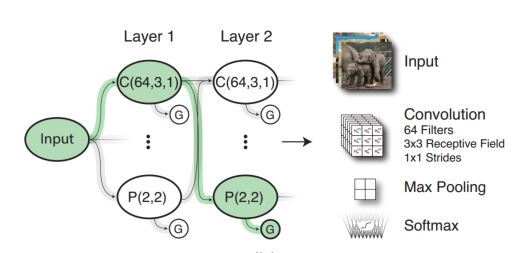
\includegraphics[width=0.85\textwidth]{adversarial_learning/images/qlearning.JPG}
    \label{fig:reinf_dnn}
    \caption{An example of reinforcement learning in deep neural networks: In green highlighted a path is shown, which the agent could select (based on MDPs) in the neural network. \cite{baker2016designing}.}
\end{figure}

\end{comment}

\subsection{Evolutionary Algorithms}
\label{evolutionaryalgorithms}
Evolutionary algorithms are based on the biological principle \textit{survival of the fittest}. Meaning, a population of individuals (e.g. solutions or scenarios) evolve through a sequence of evolutionary operators while trying to survive. After some generations, the surviving individuals represent a near-optimal solution.\\
Consequently, we want to find an individual $x \in \chi$ from an arbitrary set $\chi$ that minimizes a fitness function $f : \chi \rightarrow \mathbb{R}$. We assume that the best fitness has the lowest value. An evolutionary algorithm follows three steps \cite{michalewicz93}:
\begin{description}
   \begin{enumerate}
      \item Every $x \in \chi$ is evaluated to give some measure of its fitness score
      (Evaluation Step).
      \item A new population is formed by selecting the more fit individuals (Selection Step).
      \item Some members of the new population evolve through evolutionary operators to form new individuals. We denote $o:\mathfrak{P}(\chi)\rightarrow \mathfrak{P}(\chi)$ as the evolutionary step function so that $X_{i+1} = o(X_i)\forall i \ge 0$\\ (Alter Step).
   \end{enumerate}
\end{description}
Evolutionary operators usually follows mechanisms inspired by biological evolution. The biological operators, which are of relevance for this work are \cite{gabor19}:
\begin{description}
   \begin{itemize}
      \item \textit{recombination (rec)}: $\chi \times \chi \rightarrow \chi$ generates a new individual by combining parts of two given individuals.
      \item \textit{mutation (mut)}: $\chi \rightarrow \chi$ generates a new individual by making small changes in given individual.
      \item \textit{migration (mig)}: $\chi$ generates a random individual $mig \in \chi$
      \item \textit{selection (sel)}: $\mathfrak{P} (\chi) \times \mathbb{N} \rightarrow \mathfrak{P}(\chi)$ returns a new population\\
      $X' = sel(X,n)$ given a population $X \subseteq \chi$, so that $X' \le n$.
   \end{itemize}
\end{description}
With these steps the population should get fitter, i.e., $min_{x \in \chi_i} f(x) \ge min_{x \in \chi_i+k} f(x)$ for sufficiently large $k$. Ideally, the population converges to the best possible fitness at some point.

\subsection{Zero-sum Markov games}
\label{zerosumgames}

Zero-sum games simulate multi agent problems. The success of one agent is always the loss of the other. For example, in a two-player zero sum game, if one Agent gets a positive reward, the opponent gets an equal negative reward. This leads to the fact that the adversaries always pursue opposite goals. Payoff matrices in zero-sum games can be described as (M, -M). \inline{evtl beispiel matrizen zero-sum }
%https://neos-guide.org/content/game-theory-basics
In 2-player general-sum games (\textit{bimatrix games}) the solution depends on M\textsuperscript{1} as well as M\textsuperscript{2}. In zero-sum games, the game can be simplified by using M or -M, the solution depends only on one of the two matrices. 2-player zero-sum games are therefore called \textit{matrix games}\cite{basics2hu1998multiagent}.

\[ 
\text{For all a\textsubscript{1}} \in A\textsubscript{1}, a \textsubscript{2} \in A\textsubscript{2}, \text{and s} \in S, R\textsubscript{1}(s, a\textsubscript{1}, a \textsubscript{2}) = - R\textsubscript{2}(s, a\textsubscript{1}, a \textsubscript{2})
\]
\\
where S is the set of states of the environment, A\textsubscript{n} is the collection of actions available to Agent n and $R\textsubscript{i}:S\times A\textsubscript{1}\times A\textsubscript{2} \Rightarrow \mathbb{R}$ is each agents reward function,  given the immediately expected reward obtained by agent \textit{i} for each selection of action sets that the group of agents could make in any state\cite{basics1littman1994markov}.\\
In a two-player zero sum game, there is actually only one reward function $R\textsubscript{1}$. Agent 1 tries to maximize it and Agent 2 tries to minimize it. Hence, zero-sum games are called adversarial or fully-competitive \cite{basics1littman1994markov}.\\
If both agents converge, we speak of a Nash Equilibrium.
In a Nash equilibrium, also called the \textit{saddle point}, each agent's choice is the best answer to the other agent's choice, resulting in no agent being able to obtain rewards through unilateral deviation\cite{nashgharesifard2013distributed, basics2hu1998multiagent}.



\section{Adversarial Training}
\label{adv_training}

%----------Introduction-------------

\begin{comment}
- MOTIVATION
- limitations of random testing --> adversarial approach
- gap between simulation & real world
- model uncert
- adversarial learning is a system which involves focussing on the systems weaknesness
\end{comment}
\begin{comment}

- computer performance, reinforcement learning gets better
- traditional RL fails in real world --> gap between simulation & real world big & not enough training data (set)
- when prepared for real world -> agent should be trained with every potential danger/disturbance to the system
- training sets are limited
- new approach: adversarial reinforcement learning 

//Definition:
-Adversarial training: training the model to malicious input on purpose -> make it more robust to attack, unknown input and reduce test error \cite{MachineLearningAtScale}
- adversarial inputs are "blind spots" in training set \cite{harnessing_goodfellow}
- Linear nature of machine learning is the cause of this \cite{harnessing_goodfellow}
- Agent learns to operate in the presence of a destabilizing adversary -> the adversary agent learns an optimal destabilizing policy --> becomes the "perfect" enemy and generates training data better & broader than a human generated one

-

\end{comment}



Many reinforcement learning based approaches tend to fail in real life since the gap between simulation and real-world implementation is very large. If an agent is to be trained for the real world, it should be prepared for every possible external influence and danger, because human life could be at stake. According to Pinto et al. \cite{robustPinto2017Mar} there are two ways to perform policy learning for physical tasks: Training in the real-world which is expensive, dangerous and time-intensive. The second method is to simulate the tasks and later transfer the learned policy into the real world. But the simulated environment is generally identical to the real world and therefore the gap still exists. In addition, training sets taken from human experience are often limited and overlook such adversarial inputs, causing overfitting \cite{robustPinto2017Mar}. According to Goodfellow et al. \cite{harnessing_goodfellow}, the reason for this behavior is the linear nature of neural networks and adversarial inputs can be "blind spots" in the training set.\\
\\
The aim of the Adversarial Learning approach is to make the trained agent more robust against attacks and unknown inputs by training the model intentionally with critical input. In addition, the test error should be minimized \cite{MachineLearningAtScale}.
The complexity of an agent strongly depends on the complexity of the environment in which the agent operates. The greater and more difficult the influences of the environment, the more complex it becomes for the agent to achieve its goal \cite{environmentBansal2017Oct}.
In order to make the environment more arduous, a destabilizing unit is set against the agent. The enemy learns an optimal destabilizing policy and thus becomes the "perfect" opponent \cite{robustPinto2017Mar}. Therefore, the adversary automatically generates a challenging, broad training set that could probably not be produced by humans.
There are different approaches of adversarial machine learning. In the following we will observe and compare three types. First we have a look at a general overview of what is considered to be adversarial machine learning in a multi-agent setting in section \ref{multiagent}. Next, we discuss at "Self-Play", where one agent competes against a copy of itself (\ref{selfplay}). Finally, in \ref{gans} we take a look at "General Adversarial Networks", where a generator and a discriminator work against each other in an adversarial setup.
At the end of this chapter we will compare previously discussed scenarios of \inline{checken} self-play and GANs. 
%In the comparison we will refer to zero-sum games (\ref{zerosumgames}. A zero-sum game in self-play behaves homogeneously, while in GANs we consider a heterogeneous setup. \inline{nötig?}


%----------Concepts-------------

\subsection{Multi-Agent Competition}
%phan paper training 2

Multi-Agent Competition is primarily about training an agent 1 as well as possible by means of reinforcement learning. The goal is to train him robust against all types of inconvenience.
%and to close the gap between simulation and the real world as good as possible.
%anders formulieren
To achieve this an agent 2 is applied who learns an optimal policy also via reinforcement learning to make agent A's life as difficult as possible \cite{robustPinto2017Mar}.

\subsubsection{Related work (applications of multi-agent adversarial learning)}

To help understand adversarial learning we will look at some application areas and examples where it has been used for training in a multi-agent environment.\\

Pinto et al \cite{robustPinto2017Mar} have conducted extensive experiments with simulated agents who are supposed to learn physical tasks such as running, jumping, swimming or balance. They call their approach RARL (robust adversarial reinforcement learning). Agents who perform classical reinforcement learning would limit themselves to elementary solutions to get their reward. In order to make the conditions more difficult and thus to make agent 1 robust, agent 2 was deployed. The task of this agent is to prevent the target of agent 1 from being reached. Agent 2 is able to manipulate parameters that define agent 1, such as mass, friction, etc. and also modify the environment by letting him e.g. walk on ice instead of the usual ground.
The result of their investigations was that RARL is more robust to environmental changes than classical reinforcement learning. In addition, the learned policy performs better with random initialization of the parameters. This in turn means that the training set can be more diversified because the agent is less sensitive. The framework was also more robust in the test environment against disturbances that are difficult to design during the training \cite{robustPinto2017Mar}.

"Adversarial Tetris" is another good example of adversarial machine learning \cite{tetrisRovatsou2010May}. The task of the primary agent is to handle as many lines as possible. In contrast to the classic Tetris, the tetraminoes are not randomly selected, but are chosen as inappropriately as possible by an opposing agent. Additionally the adversary and the size of the playing field varies. \inline{minmax mit alpha beta pruning}
The agent showed satisfactory results against many different combinations of opponents and fields. He also did well in subsequent test runs \cite{tetrisRovatsou2010May}.

Competitive computer games are becoming more and more realistic. The animation of character movements plays an important role. In order to make movements look "realistic", randomness is indispensable. Wampler et al. \cite{animationwampler2010character} used adversarial machine learning to simulate intelligent, forward-thinking, unpredictable movements of a character in a game. 
For this purpose, agents competing against each other were simulated, among other things to perform was the game "Tap". An agent tries to touch another agent with his hand. The running away opponent develops a policy, which has evasion as a goal.
The movements were simulated and let observe that the agents evolve human-like movements. For example, the evasive character takes many quick, small steps as soon as the catcher approaches. This gives him the opportunity to be unpredictable and to dodge to the right or left at any time.
The agents also learned to fake movements and guessed the possible strategies of the respective opponent \cite{animationwampler2010character}.

This kind of learning also makes sense in robotics. For example, robots that play football. First, robots have to run, aim, learn to shoot. However, as soon as a defender comes into play, Stone et al. \cite{roboticstone1998towards} suggested adversarial reinforcement learning could be used to improve both attackers and defenders. The defender would have the opportunity to learn to recognize in which direction the attacker is aiming. The attacker could at the same time adjust his shot path based on the defender's movements. 
Defender and attacker would thus co-develop and challenge each other with an adaptive training set \cite{roboticstone1998towards}.

\subsubsection{State explosion in Multi-Agent environments}

One problem faced when adding additional agents is that it allows the state number to grow exponentially. Learning speed is negatively affected and in many states the precise position of the opponent is not of any relevance \cite{multiuther1997generalizing}.
Describing such a large set of states individually using a value function is intractable, so a form of generalization must be used \cite{boyan1995generalization}. 
To avoid this exponential mass of states, Uther et al. \cite{multiuther1997generalizing} compared different non-generalizing and generalizing algorithms in a multi-agent environment. 
Their application case was Hexcer - a two-player multi-agent hexagonal grid soccer game. Two agents are the adversary to each other and try to score/ prevent the enemy from scoring. Their findings showed that both their generalizing algorithms (Continuous U Tree, Fitted Prioritized Sweeping) performed significantly better than the non-generalizing algorithms (Prioritized Sweeping) \cite{multiuther1997generalizing}.
%hier evtl algorithmen kurz erklären? bzw überhaupt sinnvoll?

%beispiele suchen und beschreiben!

\subsection{Self-Play, a homogeneous zero-sum scenario}
\label{selfplay}
\begin{comment}

- Dota 2 openai
    - https://openai.com/five/
    - https://openai.com/blog/openai-baselines-ppo/
    
- phan paper training 1 - agents develop motor skills
- \cite{selfplay-heinrich}  many real-world applications are in principle games

- schach?
- go?
- dota?
- physical openai

"if you arent really good - your opponent isnt either. if you are getting better - your opponent gets better" - perfect curriculum

"agent that you train in self play is useful for external task"

https://www.youtube.com/watch?v=BJi6N4tDupk

supervised learning - limited by dataset - creates ceiling of how far it can go
\end{comment}


In October 2015, the Al AlphaGo defeated European champion Fan Hui in the Go game. In March 2016, 18-time international champion Lee Sedol was beaten by AlphaGo's successor \cite{GoalphaGosilver2017mastering}. 

\begin{comment}
AlphaGo was initially trained with the help of supervised learning, fed with moves from professional players. Afterwards policy-gradient reinforcement learning was applied and the value network was taught to determine the winner of games of the policy network against itself. These networks were then combined with Monte-Carlo Tree Search to select the best possible action from the current state \cite{alphaGosilver2017mastering}.
\end{comment}

AlphaGo was initially trained with the help of supervised learning, fed with moves from professional players.
The problem with supervised learning is that the available data set usually implies an upper limit for the learning performance. Reinforcement learning, on the other hand, learns from its own experience and can advance into areas that humans may not be able to fathom. So the AI AlphaGo has managed to become superhuman and defeat the best Go players in the world, but may not have reached its full potential yet.

As a result, Deepmind developed a program called AlphaGo Zero that learned exclusively through self-play "tabula rasa". This means that the agent did not know any sample moves from expert players or could compare his own with them. Only the rules of the game were given to the agent at the beginning. Starting with random game moves, AlphaGo became the best currently existing Go player in the world (beating previously mentioned, champion defeating original AlphaGo 100-0). But not only Go, also Chess and the japanese version of it, "shogi", was mastered by the algorithm \cite{chessSilver2017mastering,GoalphaGosilver2017mastering}. 

Self-play means that the agent always plays against a copy of itself.
\inline{self-play definition}
Deepminds AlphaZero uses Monte-Carlo Tree Search \cite{montecarlobrowne2012survey} and a deep neural network that estimates the probability of winning the current player has from the active position. This neural network assumes the roles of policy network and value network in a single environment.
%monte-carlo kurz erklären?
\\
%TDgammon
Self-play is not a completely new field of research. Already in 1992 Gerald Tesauro \cite{TDGammontesauro1992practical,TD2Gammontesauro1995temporal} developed a neural net, which learned to play backgammon on world champion level. The game-learning "TD-Gammon" is a neural net that trains itself to be an evaluation-function and learn from the outcome of each game.

27 years later, on april 13, 2019, OpenAI "Five" was the first AI ever to beat a world champion in an esports game named Dota 2. In a best-of-three series, the AI won 2-0. Afterwards, OpenAI Five was made available to all Dota 2 players as opponent or team partner - the potentially largest deployment of a highly professional deep learning agent with whom people can knowingly interact. Out of 7215 games in the first three days, the AI won 99.4\%\cite{dotaOpenAI2019Jun}.

Dota 2 is a highly complicated game, much more complicated than Go. Imagine OpenAI Five as a team of five artificial neural networks, which started with no knowledge. From the bots' point of view, Dota 2 is a structure of 20,000 (compared to chess' 8x8) numbers that reflect what a human eye would see. Another essential difference to board games like chess or Go is that Dota 2 has hidden information - only a fraction of the current game board is known to the AI. 180 years of gameplay each day has played the AI against copies of itself, consuming the processing power of 128,000 CPU cores and 256 GPUs. For every game frame, OpenAI's training system called "Rapid" awards a positive reward when something good has happened and a negative reward when something bad has happened. OpenAI's Proximal Policy Optimization \cite{ppoSchulman2019Mar} is then applied and results in actions immediately before a positive reward being rated better than those prior to a negative reward \cite{dotaOpenAI2019Jun}.
\inline{hier paper openai physics / sumoringer usw}

Das Team von OpenAI hat im Übrigen herausgefunden, dass self-play bei simulierten Agenten dazu führen kann, dass physische Fähigkeiten wie Ducken, faking, Kicken, Fangen, usw. ohne Vorwissen erlernt werden kann. So stehen beispielsweise zwei Agenten auf einer runden Plattform und müssen versuchen, sich gegenseitig von der Plattform zu stoßen (environment "Sumo"). Der humanoide Agent lernte, mit dem Kopf zu stoßen und dem angreifenden Gegner am Rand der Plattform auszuweichen, um ihn ins Leere laufen zu lassen.\\
Am Anfang des Trainings ein dichter reward \inline{quelle} für einige Schritte vergeben, um dem Agenten grundlegende motorische Fähigkeiten wie Laufen oder Stehen beizubringen. Für die policies wurden multilayer perceptron (MLP) und long short-term memory (LSTM) verwendet und verglichen.


%evtl checker by samuel

%evtl TD-Gammon




\subsubsection{GANs}
\label{gans}
\begin{comment}

    -look at gradient descent --> adjust weights in specific direction, move down the gradient
    - discriminator (classifier) (supervised learning) (0-1) fake or real?
        --> if discriminator says fake -> negative reward for generator
    - generator (random noise) -> generates new sample
    --> competetive game (one wants error rate to be high - one wants it to be low)

    - as the descriminator gets better, the generator has to get better aswell
\end{comment}



 \subsection{Comparison}
\label{adv_comparison}
 
 \begin{comment}
 
- vergleichen, wie es sich nach jeder trainingsrunde verhält: bei self-play wird der bessere genommen - bei GANs muss zb diskriminator "warten" ? 
 
 - algorithmen vergleichen - entscheidung, update, 
 
 - homogenes gameplay bei Go: beide agents haben gleiche aufgabe.
 
 - heterogenes gmaeplay bei GANs: Spieler verfolgen genau entgegengesetzte Ziele.
 
 
 - GANs sind wohl der allgemeinere Fall - aber warum sollte man dann Self-Play verwenden?
- Bietet ein Ansatz (theoretische) Garantieen, die ein anderer Ansatz nicht hat? (Garantie, dass der Gegner immer gleich gut ist beim self-play zb) 
- Was ist effizienter und leichter zu implementieren? 
- Gibt es Beispiele für Agentensysteme oder praktische Anwendungsfälle, in denen das eine mehr Sinn macht als das andere (abgesehen vom offensichtlichen Fall homogen vs. heterogen).
 
 
\end{comment} 
 
 
 To close the training chapter, self-play (\ref{selfplay}) and GANs (\ref{gans}) will now be compared.
 For our analysis we consider the zero-sum game (\ref{zerosumgames}) as a setting. 
 %The comparison is interesting because the self-play operates as a homogeneous zero-sum game, while GANs are a heterogeneous entity. This means that in self-play both agents logically follow the same goal, while in GANs opposite goals are pursued.\\

%GANs sind wohl der allgemeinere Fall - aber warum sollte man dann Self-Play verwenden?

\subsubsection{When to use which approach?}
%own experience
%no supervision of data
%no dataset

The first question we will deal with is: When is what type of adversarial learning applied?
Of course, what is decisive here is which goal is pursued and, above all, in which environment the agent is to be trained.\\

%GAN's general case:
GANs in our case represent the classical approach (we refer to it as the classical approach), where the primary goal is to train an agent and to make the training constantly more difficult by deploying an opposite agent. We call this type of adversarial training, in which rewards are given for opposite goals, heterogeneous. For instance the examples mentioned in \ref{multiagent}.
%This is to increase the complexity of the desired agent \ref{multiagent}. One must mention, however, that the opponent of the trained algorithm was at the end only a helpful means to the end


%When self-play?
Zero-sum games in which two players pursue the same goal and have the same environment and resources are particularly suitable for self-play. We're talking about homogeneous adversarial training here. Examples would be AlphaGo Zero, both agents have one playing field, the same number of stones and one goal: biggest territory at the end. Equivalent to this are for example Dota 2 (one map, destruction of the opponent's fortress) or Chess (a board, checkmate as target).
In principle, all applications implemented as self-play could also be implemented as a classical adversarial approach. In Go, for example, two neural networks could play against each other, but not learn in a coordinated way. On the other hand, not every classical adversarial training could also take place as self-play. So the idea of implementing two generators in one GAN would make little sense. A discriminator would still be needed to evaluate the generated data.

Translated with www.DeepL.com/Translator

\subsubsection{What do the approaches promise /what are the drawbacks?}


\subsubsection{What do the }
\section{Concepts of Co-Evolutionary Testing}
\label{testing}
Learning systems are often used in safety critical domains, where potential failures can have catastrophic consequences. Therefore, it is essential to evaluate said architectures thoroughly to minimize risk and maximize safety. Due to their limitations, traditional random testing algorithms can not ensure minimum failure probability (see \ref{problem}). To address this issue, the following chapter focuses on concepts of co-evolutionary testing. Section \ref{avf} and \ref{coevolution} including their subsections will describe and assess two state of the art co-evolutionary evaluation methods.

%----------Problem-------------

\subsection{Limitations Of Random Testing}
\label{limitations}
As mentioned before, a thorough testing process is necessary before integrating the learning system in a safety critical domain. When using a traditional random testing algorithm, usually the confidence that the failure rate of a policy is below $\epsilon$ requires at least $1/\epsilon$ testing episodes. This might be inefficient and time-intensive. For example in a autonomous driving domain. If there is a greater failure probability than $\epsilon = 10^{-8}$ per mile, meaning the car would crash at least once in 100 million miles, it would not be brought on the market. In order to achieve reasonable confidence, the manufacturer would need to test-drive the car for at least $10^{-8}$ miles, which may be prohibitively expensive \cite{uesato18}. Additionally, we don't exactly know how the environment will behave unless all possibilities are tried. For a huge variety of scenarios this process can get unreasonable. The agent can be trained and tested on random samples from the scenario space. However, this might cause the agent to specialize on the average scenario, which might provoke incidents. Hence, the agent is still not fully dependable \cite{gabor19}. To overcome these obstacles, a novel testing approach is needed.

\subsubsection{Intelligence Tests}
\label{intelligence}
Hernández-Orallo \& Dowe \cite{orallo10} introduced the \textit{anytime intelligence test}. This test adapts to the current intelligence of the system. When the systems' intelligence changes, the test adjusts itself. The basic idea is to initially test the agent on easy levels. When the agent succeeds it needs to overcome a harder environment. A set of environments of different complexity is required to evaluate the agent. These environments were created on a theoretical base (e.g. Solomonoff prediction) with a determined a priori complexity. This approach tests the intelligence of a system, but can not thoroughly test a learning system. The autonomous car, for example, still needs to see a unreasonable amount of scenarios.\\
Insa-Cabrera et al. \cite{cabrera11} used the idea of \cite{orallo10} to construct a general intelligence test for the evaluation of reinforcement learning algorithms. Here, all possible environments are ordered by their Kolmogorov complexity from which a set of samples is drawn. With this set, adaptive tests can be constructed which can be used to evaluate an agent. However, this concept only examines well-known properties of Q-learning. It is not known if this method works for other reinforcement learning algorithms, too. The problem, that all possible environments are needed, still exists.

\subsubsection{Co-Evolution}
\label{coevolutio}
Gabor et al. \cite{gabor18} claim that all steps related to testing adaptive systems need to become self-adaptive. In order to achieve adaptive quality assurance, they introduced the paradigm of scenario coevolution. Instead of randomly creating test scenarios, this architecture describes a set of test cases, that evolves in parallel to the behavior of the system. In this publication, the co-evolutionary process is applied to software engineering, where the test wants to find bad behavior in the productive code, whereas the productive code tries to avoid making mistakes.\\
The testing algorithm and the productive code competitively co-evolve. Wang et al. \cite{wang19} used this concept to generate increasingly complex and diverse learning environments through evolutionary strategies. They train a neural network controlling a walker that tries to optimize for an environment. These environments can be modified by the algorithm (POET - \textbf{P}aired \textbf{O}pen-\textbf{E}nded \textbf{T}railblazer) to create increasingly complex scenarios, the agent needs to solve. This way, POET managed to produce a diverse range of highly developed behaviors for a big range of environments. Unfortunately, this concept can only be used to train the agent. The testing problem still exists.\\
Co-evolutionary approaches in training help the agent to minimize failures. Therefore, it may seem obvious, that co-evolutionary techniques can be used for an efficient evaluation of reinforcement learning systems.

%----------Evaluation-------------

\subsection{Failure Probability Predictor (AVF)}
\label{avf}
Uesato et al. \cite{uesato18} proposed a failure probability predictor (AVF) for evaluating learning systems. If not stated otherwise, this chapter derives from the original paper. This architecture follows two specific tasks. To find a catastrophic failure of the agent (see section \ref{failure}) and to estimate the \textit{failure probability} up to a fixed \textit{relative accuracy} with high probability of given failure (see section \ref{risk}).\\
On both objectives, the algorithm has access to historical data and can sample from the distribution $P_X$ over initial states $X$ defined by the environment.\\
The AVF $f_*:X->[0,1]$ returns the probability of a failure given a initial condition. The estimators were assessed by the total number of experiments required and compared with 
the \textit{vanilla Monte Carlo} estimator (VMC).

\subsubsection{Failure Search}
\label{failure}


\subsubsection{Risk Estimation}
\label{risk}


%----------Concepts Of Scenario Co-Evolution-------------

\subsection{Scenario Co-Evolution}
\label{coevolution}
The Scenario Co-Evolution method by Gabor et al. \cite{gabor19} is another novel approach to tackle the issue of testing learning systems reliably. If not stated otherwise the content of this chapter derives from the original publication.\\
This concept is an instance of the general architecture of \cite{gabor18} briefly mentioned in section \ref{limitations}. The basic idea is to train an evolutionary algorithm, that co-evolves with a reinforcement learning agent and actively finds problems that are hard to solve for the agent. While the expertise of the agent evolves, the set of test instances (or \textit{scenarios}) co-evolves. After training, the co-evolutionary algorithm should return a set of hard test scenarios, that can be used for evaluating the agent.\\\\
More specifically, hard settings $x$ (or values $x$) from the scenario space $\chi$, for which the agents' performance deteriorates are wanted. Similar to Zero-sum Markov games (section \ref{zerosumgames}) two algorithms optimize against each other. While the agent tries to maximize its fitness, the co-evolutionary algorithm tries to find scenarios which minimize the agents' fitness. An evolutionary algorithm (section \ref{evolutionaryalgorithms}) that optimizes for hard settings for $x$ is used to find those the respective values for $x$. Figure \ref{fig:scenario_coevolution} shows a visual representation of the evolutionary algorithm.
\begin{figure}
  \centering
  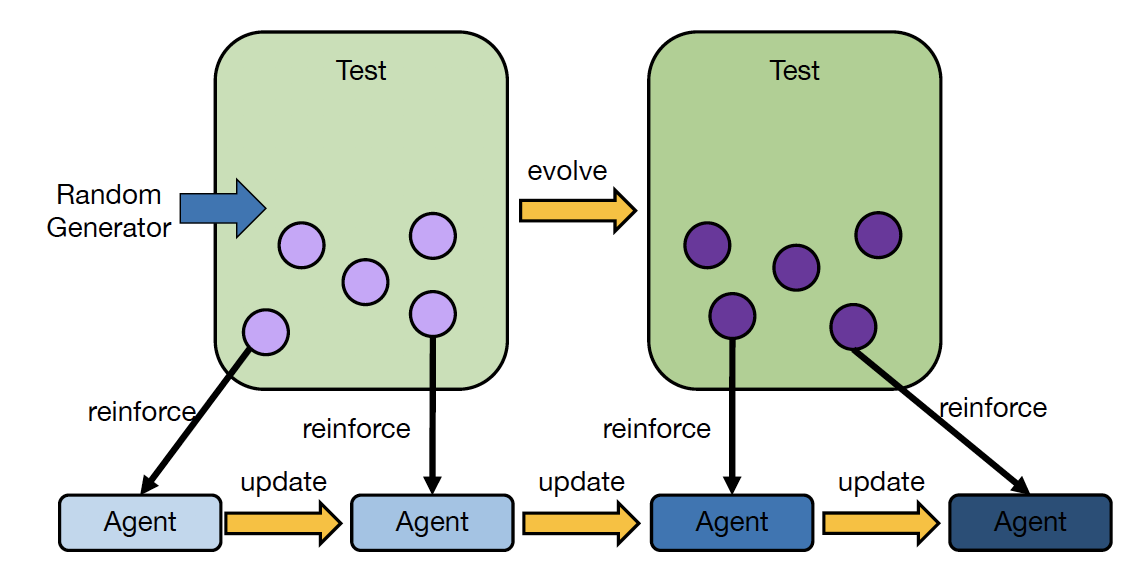
\includegraphics[width=0.85\textwidth]{adversarial_learning/images/scenario_coevolution.png}
  \label{fig:scenario_coevolution}
  \caption{Visual representation of the evolutionary process by \cite{gabor19}. First, a set of test scenarios is randomly generated. The set improves via evolution. Between evolution steps, the test data is used to train the agent. This causes the reinforcement learning agent to co-evolve with the test data.}
\end{figure}
It constructs an evolutionary process with the scenario space $\chi$. Experience samples are needed to train the agent. These are drawn using settings for $x \in \chi$ from the current population $\chi$ of the evolutionary process. After all $x \in \chi$ have been used, the evolutionary process evolves further for a few generations. In this work, the evolutionary step function for selection schemes $\sigma_1, \sigma_2, \sigma_3$ is:
\begin{equation}
X_{i+1} = o(X_i) = sel(mig_{\sigma_3}(mut_{\sigma_2}(rec_{\sigma_1}(X_i))),|X_i|)
\end{equation}
After a few generations of optimizing for hard $x$ the resulting experience sample is used to generate experience samples for the reinforcement learning agent. As mentioned, the reinforcement learning agent tries to maximize its reward, while the evolutionary process tries to minimize the fitness. The fitness $f(x)$ assigned to each $x \in \chi$ is calculated using the accumulated reward of running the current agent policy $\pi$ on the MDP $M_x$ (section \ref{mdp}). In turn, the reinforcement learning agent with the current highest fitness score is used to evaluate the hardness of the settings for $x$ for the next few generations of evolution.\\
With every evolutionary step the agent trains on harder settings from the test population. Simultaneously the fittest agent evaluates the hardness of the settings. In the end, the algorithm is able to return a set with the hardest test scenarios. When the agent can solve these hard problems, it can be assumed that it can solve easy scenarios, too. Consequently, there is no need to generate all possible scenarios. Additionally, these scenarios are not limited to the trained agent. They can be used to evaluate every agent running on the same environment.

\subsection{Comparison}
\label{comparison}
This chapter compares the \textit{failure probability predictor} (AVF) (section \ref{avf}) and the \textit{Scenario Co-Evolution} (SCoE) (section \ref{coevolution}) testing approaches. The goal of each concept is to outperform standard evaluation approaches for reinforcement learning agents by finding a more efficient method of detecting rare, catastrophic failures. While the AVF uses \textit{importance sampling} to actively search for failures and estimate the failure risk, the SCoE uses \textit{evolutionary algorithms} to evolve a set of hard test scenarios to evaluate the agent. While both architectures outperform traditional random testing methods and solve the problem of having to test the agent on every scenario, they are fundamentally different.\\\\
Both algorithms co-evolve with an agent. Because the AVF looks for failures of this specific agent, it specializes on it. Meaning, the testing algorithm cannot be used to evaluate another, independently trained agent running on the same domain.\\
SCoE however does just that. The resulting test scenarios of the SCoE are hard to solve for any other agent. Once the SCoE returns a set of test scenarios, all agents running on the same environment can be evaluated with this exact set. SCoE is a more generic and simpler way to test agents on a specific domain.\\\\
A standard random reinforcement learning agent performs worse on SCoE generated scenarios than on random generated scenarios. It shows that SCoE generated scenarios discover more catastrophic failures than traditional generated scenarios. Hence, the SCoE testing process is more reliable. Still, we simply assume, that the agent can solve easy scenarios, if it is able to overcome hard cases. The agent gets better in all scenarios by training on hard scenarios, but still does not explicitly look for failures like the AVF.\\
As already described, the AVF actively searches for failures of the agent. In comparison to a standard \textit{Vanilla Monte Carlo} (VMC) estimator, the AVF minimizes the errors in risk estimation in a fraction of the time. For example, the VMC needs 12000 episodes in a driving domain whereas the AVF minimizes the errors in risk estimation after only 2000 episodes. Additionally, the error rate of the AVF is smaller after 2000 episodes, than the VMCs error rate ever is. Unfortunately, there is no measurement of the error rate for the SCoE. Because the AVF actively searches for failures while the SCoE "only" provides hard test cases, it might lead to the assumption, that the AVF is less error-prone.\\\\
Optimization through evolutionary algorithms tend to be slow for computationally intensive problems regarding the evaluation of each problem \cite{cruz}. Importance Sampling is often used to produce fast learning algorithms \cite{chen18, schaal04}. The underlying search algorithms lead to the supposition, that AVF (with Importance Sampling) might faster per timestep than SCoE (with Evolutionary Algorithms). Unfortunately, there is no direct comparison possible.\\\\
The SCoE was used to train and test an agent trying to transport items to workstations in a comprehensible multi-agent $7 \times 8$ grid \textit{smart factory domain}. The AVF was evaluated in a continuous \textit{driving} domain, where the agent was rewarded for forward progress without crashing and in a continuous \textit{humanoid} domain, where the agent was rewarded for standing without falling. It is not known, how the AVF performs in a multi-agent domain and vice versa. At this point, we can not know, which method is a better fit for a specific type of environment.\\\\
In summary, the SCoE is a more intuitive approach, can evaluate independent agents and is proven to work great in small grid domains. The AVF might be more reliable, reduces time of searching for failures, but specializes in one agent.

\begin{comment}
Hoppla, hier gibt es aber noch was Visuelles, nämlich Abbildung~\ref{fig:karate} mit dem Karate-Graph nach \cite{zachary1977information}. 
\end{comment}


\begin{comment}
\section{Beispiel figure:}

\begin{figure}
  \centering
  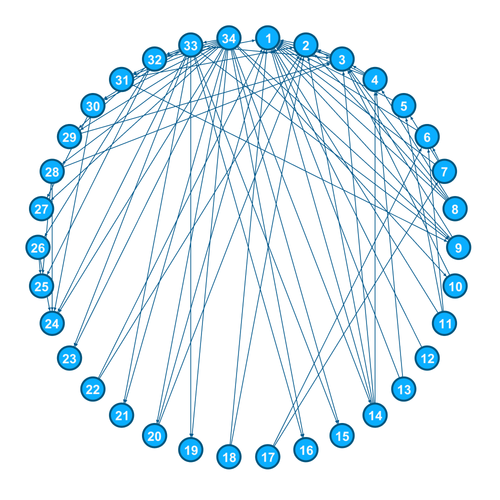
\includegraphics[width=0.85\textwidth]{images/karate}
  \label{fig:karate}
  \caption{Der Graph eines Karate-Clubs nach \cite{zachary1977information}.}
\end{figure}
\end{comment}



